% This work is made available under the terms of the
% Creative Commons Attribution-ShareAlike 4.0 license,
% http://creativecommons.org/licenses/by-sa/4.0/.
%
% Version: $Revision$

\documentclass[a4paper]{book}

\usepackage{wrapfig}
\usepackage{graphicx}
\usepackage{hyperref}
\usepackage{multirow}
\usepackage{scalefnt}
\usepackage{tikz}

% watermark -- for draft stage
\usepackage[firstpage]{draftwatermark}
\SetWatermarkLightness{0.9}
\SetWatermarkScale{5}

% Copyright (c) 2009 by the University of Waikato, Hamilton, NZ. 
% This work is made available under the terms of the 
% Creative Commons Attribution-ShareAlike 4.0 license,
% http://creativecommons.org/licenses/by-sa/4.0/.
%
% Version: $Revision: 5479 $

\newenvironment{tight_itemize}{
\begin{itemize}
  \setlength{\itemsep}{1pt}
  \setlength{\parskip}{0pt}
  \setlength{\parsep}{0pt}}{\end{itemize}
}

\newenvironment{tight_enumerate}{
\begin{enumerate}
  \setlength{\itemsep}{1pt}
  \setlength{\parskip}{0pt}
  \setlength{\parsep}{0pt}}{\end{enumerate}
}

% if you just need a simple heading
% Usage:
%   \heading{the text of the heading}
\newcommand{\heading}[1]{
  \vspace{0.3cm} \noindent \textbf{#1} \newline
}

\newcommand{\icon}[1]{\tikz[baseline=-3pt]\node[inner sep=0pt,outer sep=0pt]{\includegraphics[height=1.1em]{#1}};}


\title{
  \textbf{ADAMS} \\
  {\Large \textbf{A}dvanced \textbf{D}ata mining \textbf{A}nd \textbf{M}achine
  learning \textbf{S}ystem} \\
  {\Large Module: adams-dl4j} \\
  \vspace{1cm}
  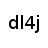
\includegraphics[width=2cm]{images/dl4j-module.png} \\
}
\author{
  Peter Reutemann
}

\setcounter{secnumdepth}{3}
\setcounter{tocdepth}{3}

\begin{document}

\begin{titlepage}
\maketitle

\thispagestyle{empty}
\center
\begin{table}[b]
	\begin{tabular}{c l l}
		\parbox[c][2cm]{2cm}{\copyright 2016-2017} &
		\parbox[c][2cm]{5cm}{
\includegraphics[width=5cm]{images/coat_of_arms.pdf}} \\
	\end{tabular}
	
\includegraphics[width=12cm]{images/cc.png} \\
\end{table}

\end{titlepage}

\tableofcontents
%\listoffigures
%\listoftables

%%%%%%%%%%%%%%%%%%%%%%%%%%%%%%%%%%%
\chapter{Introduction}
The \textit{dl4j} module makes the deeplearning4j\cite{dl4j} library available
within ADAMS.

Due to the complex nature of configuring deep belief networks and such
multi-layered neural networks, there is no graphical support for configuring
networks as such. Instead, a so-called \textit{model configurator} is used
to return a configured model. This can be achieved in two ways:
\begin{tight_itemize}
  \item \textit{Custom Java code} -- you can subclass
  \textit{AbstractModelConfigurator} (located in package \textit{adams.ml.dl4j.model})
  and implement your own parameters that are necessary for tweaking your network. This is
  done by the \textit{SimpleMultiLayerNetwork} class in that package, which
  is just a configurable version of the network describe by deeplearning4j's
  tutorial on the iris dataset.
  \item \textit{Scripting} -- taking advantage of either Groovy or Jython,
  you can use the \textit{ModelWithScriptedConfiguration} class pointing
  to your script file that generates the actual network to be trained and used.
\end{tight_itemize}

%%%%%%%%%%%%%%%%%%%%%%%%%%%%%%%%%%%
\chapter{Flow}

The following sources are available:
\begin{tight_itemize}
  \item \textit{DL4JDatasetIterator} -- outputs datasets using the specified
  dataset iterator.
  \item \textit{DL4JModelConfigurator} -- defines a deeplearning model.
  \item \textit{DL4JModelGenerator} -- generates model(s) using the specified
  generator scheme.
\end{tight_itemize}

The following transformers are available:
\begin{tight_itemize}
  \item \textit{DL4JCrossValidationEvaluator} -- cross-validates a model
  on the incoming dataset.
  \item \textit{DL4JCrossValidationSplit} -- generates sequence of train/test
  splits from the incoming dataset.
  \item \textit{DL4JDatasetAppend} -- combines multiple datasets into a single one,
  one after the other.
  \item \textit{DL4JDatasetInfo} -- outputs information about a dataset.
  \item \textit{DL4JEvaluationSummary} -- generates a summary from an Evaluation
  object/container.
  \item \textit{DL4JEvaluationValues} -- retrieves statistics from an Evaluation
  object/container and places them in a spreadsheet.
  \item \textit{DL4JModelReader} -- reads a serialized model from disk.
  \item \textit{DL4JRandomSplit} -- generates a random split on the incoming dataset.
  \item \textit{DL4JScoring} -- generates scores (= predictions) for a dataset
  using a built model.
  \item \textit{DL4JTestSetEvaluator} -- evaluates an incoming built model on a
  callable dataset.
  \item \textit{DL4JTrainModel} -- builds a model obtained from a callable model
  configurator on the incoming dataset.
  \item \textit{DL4JTrainTestSetEvaluator} -- trains and evaluates a model obtained
  from a callable model configurator on the incoming train/test set container.
\end{tight_itemize}

The following sinks are available:
\begin{tight_itemize}
  \item \textit{DL4JModelWriter} -- saves a model to disk using serialization.
\end{tight_itemize}

The following conversions are available:
\begin{tight_itemize}
  \item \textit{DL4JConfiguratorToModel} -- obtains an actual model from a configurator.
  \item \textit{DL4JDataSetToSpreadSheet} -- turns a DL4J DataSet into a SpreadSheet.
  \item \textit{DL4JJsonToModel} -- turns a JSON\cite{json} object into a model.
  \item \textit{DL4JModelToJson} -- turns a model into its JSON\cite{json} representation.
  \item \textit{DL4JModelToSpreadSheet} -- turns the parameters of a model into a spreadsheet.
  \item \textit{DL4JModelToString} -- turns the parameters of a model into a simple string representation.
  \item \textit{DL4JModelToJson} -- turns a model into its JSON\cite{json} representation.
  \item \textit{DL4JModelToYaml} -- turns a model into its YAML\cite{yaml} representation.
  \item \textit{DL4JYamlToModel} -- turns a YAML\cite{yaml} string into a model.
  \item \textit{NDArrayToSpreadSheet} -- turns a NDArray into a spreadsheet.
  \item \textit{SpreadSheetToDL4JDataSet} -- turns a spreadsheet into a DL4J DataSet.
\end{tight_itemize}

%%%%%%%%%%%%%%%%%%%%%%%%%%%%%%%%%%%
\section{Iteration listeners}
By default, building models does not provide any insight into how the building
is going. However, DL4J offers iteration listeners that can shed some light
on the build process.

These listeners can be attached to the following actors:
\begin{tight_itemize}
  \item DL4JCrossValidationEvaluator
  \item DL4JTrainModel
  \item DL4JTrainTestSetEvaluator
\end{tight_itemize}

The following schemes for configuring iteration listeners are available:
\begin{tight_itemize}
  \item \textit{NullListener} -- does nothing
  \item \textit{CallableActorScoreListenerConfigurator} -- forwards double array
  of iteration/score to the specified callable actor (e.g., for plotting)
  \item \textit{InMemoryStatsListenerConfigurator} -- stores statistics in memory
  and allows accessing them via a web interface on \url{http://localhost:9000/train}{}
  \item \textit{ScoreIterationListenerConfigurator} -- simple logging of
  statistics in console
\end{tight_itemize}

\begin{figure}[htb]
  \centering
  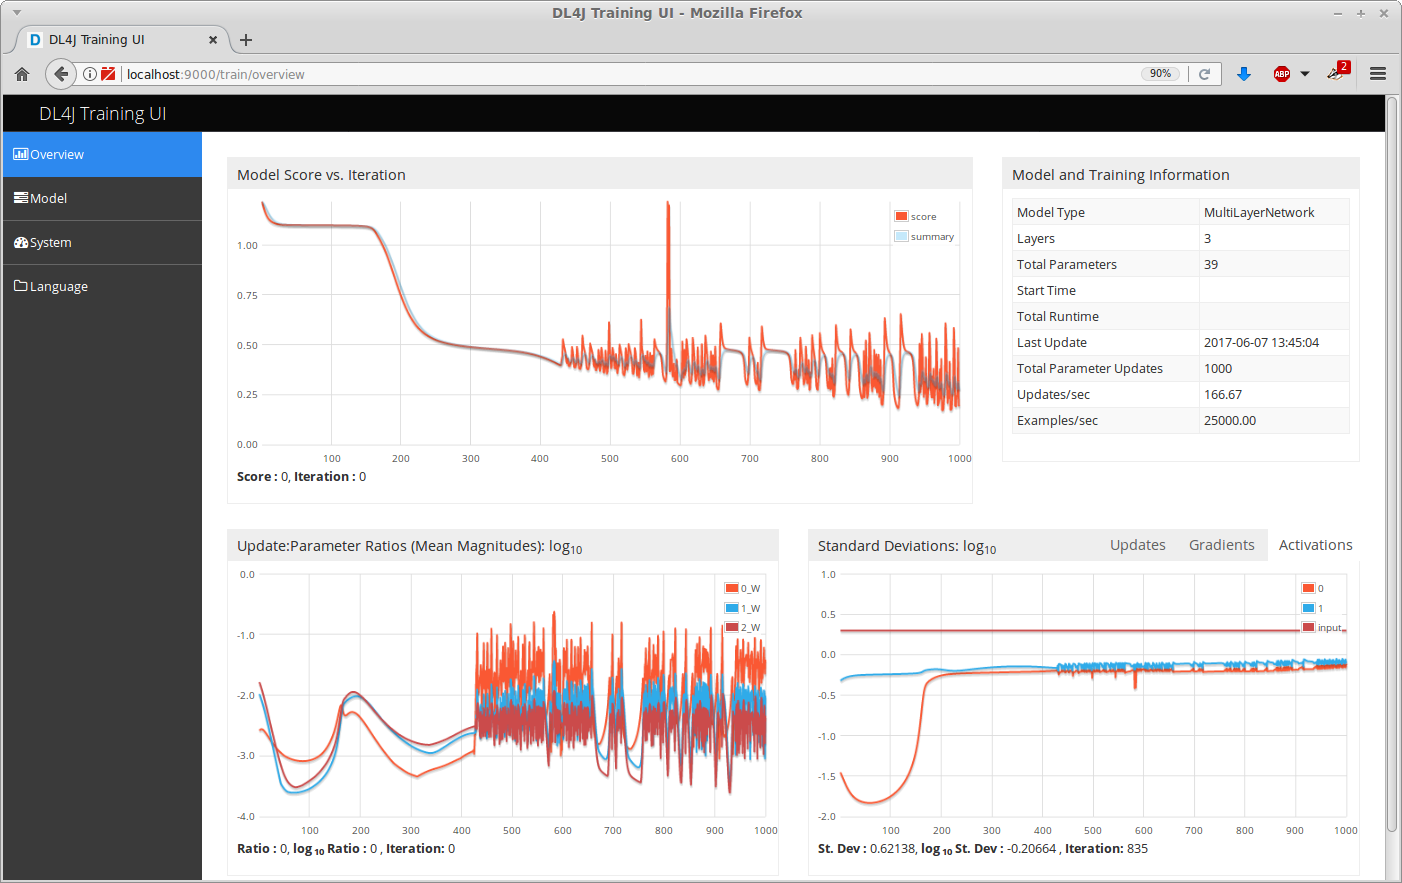
\includegraphics[width=12.0cm]{images/stats_iteration_listener.png}
  \label{stats_iteration_listener}
\end{figure}


%%%%%%%%%%%%%%%%%%%%%%%%%%%%%%%%%%%
\chapter{CUDA Support}
By default, dl4j (actually nd4j\cite{nd4j}) uses the CPU for linear algebra.
However, if you have CUDA installed, you can switch to GPU computation by
adding another dependency in your \textit{pom.xml} file.

The current version of nd4j supports CUDA\cite{cuda} versions
7.5 and 8.0 at the time of writing\footnote{Check Maven Central for updated
artifacts using \url{http://search.maven.org/\#search\%7Cga\%7C1\%7Cnd4j-cuda}{}},
and requires you to specify which one you have.
For example, if you have CUDA v7.5 installed, then you need to define the
\textit{artifactId} like this:

\begin{verbatim}
    <dependency>
      <groupId>org.nd4j</groupId>
      <artifactId>nd4j-cuda-7.5</artifactId>
      <version>${nd4j.version}</version>
    </dependency>
\end{verbatim}

If you do not compile your own project, but simply use ADAMS releases/snapshots,
then you can simply download the appropriate version of the CUDA libraries. E.g.,
for CUDA 7.5, this is \textit{adams-dl4j-cuda-7.5-libs}. Just add all the
files in the \textit{lib} directory of this archive to the one of your ADAMS
installation to enable CUDA support. But be aware that ADAMS will only work
if you have CUDA support on the machine that you are running it on (a
design drawback of deeplearning4j, unfortunately).


%%%%%%%%%%%%%%%%%%%%%%%%%%%%%%%%%%%
\chapter{OpenBLAS}
By default, OpenBLAS determines automatically how many threads to use for
speeding up the computing. However, you can use the following environment
variable to manually set the number of
threads\footnote{\url{https://deeplearning4j.org/native}{}}:
\begin{verbatim}
OMP_NUM_THREADS
\end{verbatim}
\textbf{NB:} This should be the number of \textit{actual} cpus/cores.
Systems with hyper-threading support will report multiples of this number.


%%%%%%%%%%%%%%%%%%%%%%%%%%%%%%%%%%%
\chapter{Intel MKL}
Intel provides high-performance BLAS libraries for download as well\cite{mkl}:

After installation, you have to add the libraries to your environment
variables for deeplearning4j to pick up.

\noindent First, locate the directory that contains the MKL runtime library:
\begin{tight_itemize}
  \item Linux/OSX: \texttt{libmkl\_rt.so}
  \item Windows: \texttt{mkl\_rt.dll}
\end{tight_itemize}

\noindent Second, add this directory to your environment variables:
\begin{tight_itemize}
  \item Linux/OSX: add the path to \texttt{LD\_LIBRARY\_PATH}
    \begin{verbatim}
    export LD_LIBRARY_PATH=$LD_LIBRARY_PATH:/path/to/mkl_rt
    \end{verbatim}
  \item Windows: add the path to your \texttt{\%PATH\%} variable, either
  through the control panel or on the command prompt:
    \begin{verbatim}
    set PATH=%PATH%:path\to\mkl_rt
    \end{verbatim}
\end{tight_itemize}


%%%%%%%%%%%%%%%%%%%%%%%%%%%%%%%%%%%
% Copyright (c) 2009-2012 by the University of Waikato, Hamilton, NZ. 
% This work is made available under the terms of the 
% Creative Commons Attribution-ShareAlike 4.0 license,
% http://creativecommons.org/licenses/by-sa/4.0/.
%
% Version: $Revision$

\begin{thebibliography}{999}
	% to make the bibliography appear in the TOC
	\addcontentsline{toc}{chapter}{Bibliography}

    % references
	\bibitem{adams}
		\textit{ADAMS} -- Advanced Data mining and Machine learning System \\
		\url{https://adams.cms.waikato.ac.nz/}{}
		
	\bibitem{heatmap}
		\textit{Heat map} -- WikiPedia article \\
		\url{http://en.wikipedia.org/wiki/Heat_map}{}

\end{thebibliography}


\end{document}
